\documentclass{article}
\usepackage[utf8]{inputenc}
\usepackage[margin=1in]{geometry}
\usepackage[table]{xcolor} 
\usepackage{changepage}
\usepackage{titling}
\usepackage{amsmath}
\usepackage{amsfonts}
\usepackage{array}
\usepackage{amssymb}

\usepackage{tikz}
\usetikzlibrary{automata, positioning}

\droptitle = -1in

% For setting page numbering, but you've already disabled it.
\setlength{\parindent}{0cm}
\pagenumbering{gobble}

\title{Homework 2}
\author{Seven Lewis}
\date{4/12/24}


% Defining custom commands for colored text
\newcommand{\problem}[1]{\noindent\textcolor{black}{#1}}
\newcommand{\solution}[1]{\noindent\textcolor{red}{#1}}

% Alternatively, defining environments for problems and solutions
\newenvironment{Problem}
{\noindent\color{black}}
{\newline}

\newenvironment{Solution}
{\noindent\color{red}}
{\newline}

\begin{document}

\maketitle

%%%%%%%%%%%%%%%%%%%%%%%%%%%%%%%%%

\section*{1. True or False}
\problem{1) The set $\{(1,1),(2,2),(3,3),(2,3)\}$ is a function.}

\solution{False}

\problem{2) Every regular language can be recongized by a deterministic finite automaton (DFA).}

\solution{True}

\problem{3) The fuction $f: \mathbb R \rightarrow \mathbb R$ defined by $f(x) = x^2 + 1$ is surjective.}

\solution{False}

\problem{4) Nondeterminist finite automaton (NFA) are more powerful than DFAs in terms of the
types of languages they can recongize.}

\solution{False}

\problem{5) The function $f: \mathbb R \rightarrow \mathbb R$ defined by $f(x) = x^3 - x$ is
injective.}

\solution{False}

\problem{6) Every NFA can be converted into an equivalent DFA}

\solution{True}

\problem{7) Let $R$ be the relation on the set $\{1,2,3,4\}$ such that $R =\{(1,2),(2,3),(3,1)\}$.
The relation $R$ is both reflexive and symmetric.}

\solution{False}

\problem{8) A given string from a regular expression can always be converted to a NFA.}

\solution{True}

\problem{9) The relation $R = \{(a,b) | a \text{ is younger than } b\}$ on the set of all people.
$R$ is Reflexive.}

\solution{False}

\problem{10) A DFA can use empty string ($\varepsilon$) transitions.}

\solution{False}

\vspace*{22em}

\section*{2. }

\begin{Problem}
    Prove using mathematical induction that for all integers $n \geq 1$:

    $$1 + 4 + 7 + \dots + (3n - 2) = \frac{n(3n-1)}{2}$$
\end{Problem}


\begin{Solution}
    Proof:

    \phantom{ }

    \begin{adjustwidth}{2em}{0em}
        \textbf{Basis Step: } $n = 1$

        \phantom{ }

        \begin{adjustwidth}{2em}{0em}
            $\displaystyle (3(1) - 2) = \frac{(1)(3(1) - 1)}{2}$

            \phantom{ }

            $\displaystyle 1 = 1 \hspace*{1em} \checkmark$ True.
        \end{adjustwidth}

        \phantom{ }

        \textbf{Inductive Step: } $n = k + 1$

        \phantom{ }

        \begin{adjustwidth}{2em}{0em}
            Assume $\displaystyle 1 + 4 + 7 + \dots + (3k - 2) = \frac{k(3k-1)}{2}$
            
            \phantom{ }

            Observe that: 

            \phantom{ }

            \hspace*{4.8em}$\displaystyle 1 + 4 + 7 + \dots + (3(k+1) - 2) = $

            \phantom{ }

            $\displaystyle 1 + 4 + 7 + \dots + (3k - 2) + (3(k+1) - 2) = $
            
            \phantom{ }

            \hspace*{6.75em}$\displaystyle \frac{k(3k-1)}{2} + (3(k+1) - 2) = $

            \phantom{ }

            \hspace*{6.25em}$\displaystyle \frac{k(3k-1) + 2(3(k+1)-2)}{2}= $

            \phantom{ }

            \hspace*{9.25em}$\displaystyle \frac{(3k^2-k) + (6k+2)}{2}= $

            \phantom{ }

            \hspace*{11.45em}$\displaystyle \frac{(k+1)(3k+2)}{2} = \frac{(k+1)(3(k+1)-1)}{2}$

        \end{adjustwidth}

        \phantom{ }

        Therefore, $\displaystyle 1 + 4 + 7 + \dots + (3(n+1) - 2) = \frac{(n+1)(3(n+1)-1)}{2}$
        for all integers $n \geq 1$.
    \end{adjustwidth}

    \phantom{ }
\end{Solution}

\vspace*{16em}

\section*{3.}

\begin{Problem}
    Convert the following NFA to a DFA.

    \phantom{ }

    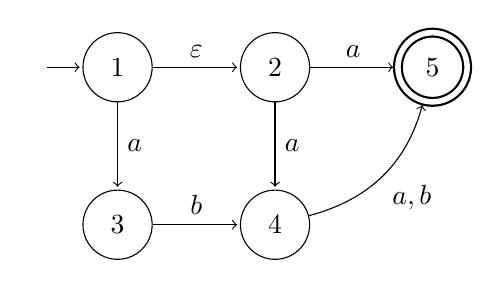
\begin{tikzpicture}[shorten >=1pt, node distance=2cm, on grid, auto, initial text =]
        \node[state, initial]   (1)                 {$1$};
        \node[state]            (2) [right=of 1]    {$2$};
        \node[state]            (3) [below=of 1]    {$3$};
        \node[state]            (4) [right=of 3]    {$4$};
        \node[state, accepting, thick, double, double distance=2pt] (5) [right=of 2] {$5$};
        
        \path[->]
        (1) edge node {$\varepsilon$}   (2)
        (1) edge node {$a$}             (3)
        (2) edge node {$a$}             (5)
        (2) edge node {$a$}             (4)
        (3) edge node {$b$}             (4)
        (4) edge [bend right] node[swap] {$a,b$}           (5);
     \end{tikzpicture}
\end{Problem}



\phantom{ }

\begin{Solution}
    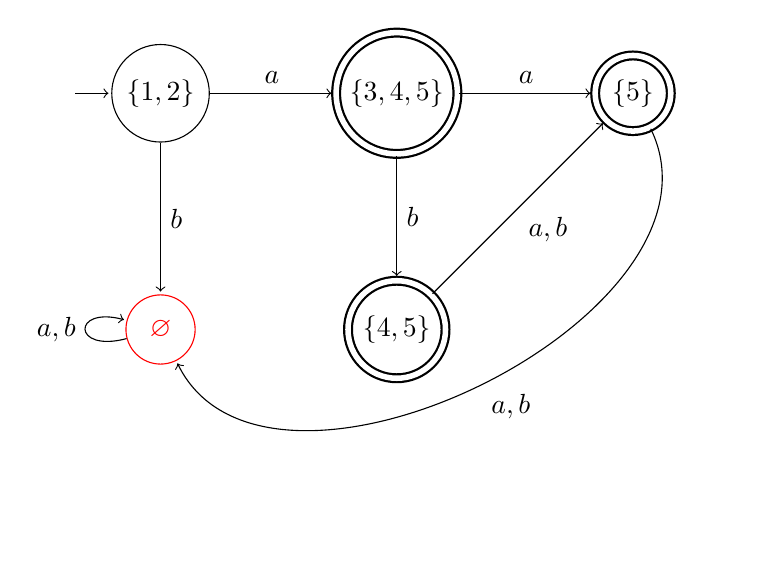
\begin{tikzpicture}[shorten >=1pt, node distance=3cm, on grid, auto, initial text =]
        \node[state, initial]   (q_1)                       {$\{1,2\}$};
        \node[state, accepting, thick, double, double distance=2pt]            (q_2) [right=of q_1]        {$\{3,4,5\}$};
        \node[state, accepting, thick, double, double distance=2pt] (q_3) [right=of q_2]        {$\{5\}$};
        \node[state,red] (q_4) [below=of q_1] {$\varnothing$};
        \node[state, accepting, thick, double, double distance=2pt] (q_5) [right=of q_4] {$\{4,5\}$};

        \path[->]
        (q_1) edge node {$a$} (q_2)
        (q_2) edge node {$a$} (q_3)
        (q_1) edge node {$b$} (q_4)
        (q_4) edge [loop left] node {$a,b$} ()
        (q_2) edge node {$b$} (q_5)
        (q_5) edge node[swap] {$a,b$} (q_3)
        (q_3) edge [bend left=90] node {$a,b$} (q_4)
        ;
    \end{tikzpicture} 
\end{Solution}

\section*{4.}

\begin{Problem}
    Convert the following regular expression to an NFA: $bb(ab)^*aa$
\end{Problem}

\begin{Solution}
    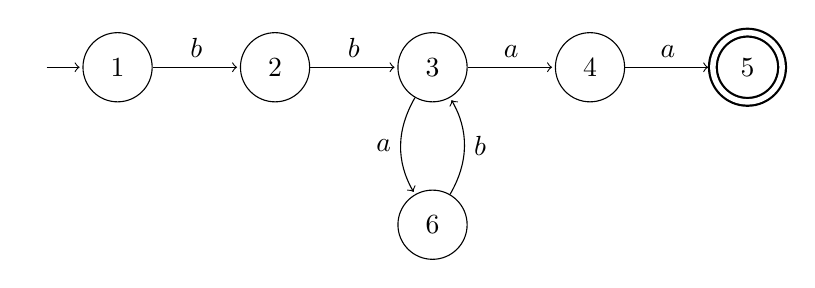
\begin{tikzpicture}[shorten >=1pt, node distance=2cm, on grid, auto, initial text =]
        \node[state, initial]   (1)                     {$1$};
        \node[state]            (2)[right=of 1]         {$2$};
        \node[state]            (3)[right=of 2]         {$3$};
        \node[state]            (4)[right=of 3]         {$4$};
        \node[state, accepting, thick, double, double distance=2pt]            (5)[right=of 4]         {$5$};
        \node[state]            (6)[below=of 3]         {$6$};

        \path[->]
        (1) edge node {$b$} (2)
        (2) edge node {$b$} (3)
        (3) edge node {$a$} (4)
        (4) edge node {$a$} (5)
        (3) edge [bend right] node[swap] {$a$} (6)
        (6) edge [bend right] node[swap] {$b$} (3)
        ;
    \end{tikzpicture}
\end{Solution}



\end{document}